% Poster Template for the Okinawa Institute of Science and Technology (OIST)
% Created by Jeremie Gillet on June 2019

\documentclass[
    a0paper, % Size of poster
    landscape, % Orientation
    fontscale=0.3 % General scaling for fonts, increase the number for smaller fonts (considered removing text first)
    ]{baposter}

% Graphics
\usepackage{graphicx} % Required for including images
\graphicspath{{figures/}} % Directory in which figures are stored

% Add any packages you need here
\usepackage{amsmath} % For typesetting math
\usepackage{vwcol}
\usepackage{enumitem} % Used to reduce itemize/enumerate spacing


% Defining colors
\selectcolormodel{HTML}
\definecolor{OIST}{HTML}{C80019} 
\definecolor{grey}{RGB}{0.06, 0.05, 0.03}
\definecolor{DarkRed}{RGB}{100,0,10}

% Changing fonts
\usepackage{palatino} % Use the Palatino font

% Starting document, feel free to change the style of headers and boxes
% Documentation can be found here: http://www.brian-amberg.de/uni/poster/
% Unfortunately it is not very complete
\begin{document}
\begin{poster}{ % General poster options
    columns=4, % Number of columns, maximum 6
    headerborder=closed, % Adds a border around the header of content boxes
    colspacing=1em, % Column spacing
    background=none, % No background
    borderColor=OIST, % Border color
    headerColorOne=white, % Background color for the header in the content boxes (left side)
    headerColorTwo=OIST, % Background color for the header in the content boxes (right side)
    headerFontColor=grey, % Text color for the header text in the content boxes
    boxColorOne=white, % Background color of the content boxes
    textborder=roundedleft, % Format of the border around content boxes, can be: none, bars, coils, triangles, rectangle, rounded, roundedsmall, roundedright or faded
    eyecatcher=true, % Set to false for ignoring the left logo in the title and move the title left
    headerheight=0.1\textheight, % Height of the header
    headershape=roundedright, % Specify the rounded corner in the content box headers, can be: rectangle, small-rounded, roundedright, roundedleft or rounded
    headerfont=\Large\bf\textsc, % Large, bold and sans serif font in the headers of content boxes
    linewidth=2pt, % Width of the border lines around content boxes
} 
{
\includegraphics[height=4em]{logo.jpg}} % First logo on the left
{\bf\textsc{Title of the Poster}\vspace{0.5em}} % Poster title
{\textsc{\{ List of Authors \} \hspace{12pt} OIST Graduate University, Japan}} % Author names and institution
{
\includegraphics[height=4em]{logo.jpg}} % Second logo on the right


%----------------------------------------------------------------------------------------
%	Abstract
%----------------------------------------------------------------------------------------


\begin{posterbox}[
    name = abstract,  % Name for alignment 
    column = 0, % Column 
    ]{1. Abstract}
Gridworlds are a popular and powerful test-bed for artificial intelligence (AI) algorithms, especially in reinforcement learning and associated AI safety problems. To describe how AI agents behave in such gridworlds, we consider gridworlds as reconfigurable systems and construct their state complexes. These state complexes reveal the underlying structures and patterns in the system's possible reconfigurations. This work incorporates the concepts of gridworlds, reconfigurable systems, and state complexes to show structures and patterns found in the state complexes of example gridworlds.

%\vspace{0.3em} % When there are two boxes, some whitespace may need to be added if the one on the right has more content
\end{posterbox}

%----------------------------------------------------------------------------------------
%	REFERENCES
%----------------------------------------------------------------------------------------

\begin{posterbox}[
    name = references,  % Name for alignment 
    column = 0, % Column 
    above = bottom, % Alignment
    ]{References}
    \renewcommand{\section}[2]{} % Get rid of the default "References" section title
    \nocite{*} % Insert publications even if they are not cited in the poster
    \bibliography{Bibliography}
    \bibliographystyle{abbrv}
\end{posterbox}


%----------------------------------------------------------------------------------------
%	FUTURE RESEARCH
%----------------------------------------------------------------------------------------

\begin{posterbox}[
    name = futureresearch,  % Name for alignment 
    column = 1, % Column 
    span = 2,
    aligned=references,
    above=bottom
    ]{6. Future Research}
We are currently exploring patterns and theoretical aspects of state complexes that hold across gridworlds of arbitrary size, geometry, and labelling. For example, an upper bound for the total number of states of a gridworld without objects is $\binom{n}{k}$ where $n$ is the total number of non-\textcolor{gray}{floor} and non-wall labels and $k$ is the total number of \textcolor{green}{agent} labels. Such information may be useful to incorporate into AI algorithms or for analysis of the efficiency, accuracy, or safety of such algorithms in gridworlds.
\end{posterbox}

%----------------------------------------------------------------------------------------
%	CONTACT INFORMATION
%----------------------------------------------------------------------------------------

\begin{posterbox}[
    name = contact,  % Name for alignment 
    column = 3, % Column 
    aligned=references,
    above=bottom
    ]{Contact Information}

\begin{vwcol}[widths={0.3,0.7},sep=.8cm, justify=flush,rule=0pt,indent=1em] 
    
\includegraphics[width=0.25\textwidth]{QR-code.png}
    \begin{description}[noitemsep]
    \item[] 
    \item[Web] tfburns.com
    \item[Email] thomas.burns@oist.jp
    \item[Phone] +81 (0)90 6863 7039
    \end{description}
\end{vwcol} 
\end{posterbox}


%----------------------------------------------------------------------------------------
%	Gridworlds
%----------------------------------------------------------------------------------------

\begin{posterbox}[
    name = grid,  % Name for alignment 
    column = 0, % Column 
    above=references,
    below=abstract
    ]{2. Gridworlds}
\hspace{1em}
\begin{center}
    \quad \tikz\draw[green,fill=green] (0,0) circle (.5ex); agent
    \quad \tikz\draw[blue,fill=blue] (0,0) circle (.5ex); object
    \quad \tikz\draw[gray,fill=gray] (0,0) circle (.5ex); floor
    \quad \tikz\draw[black,fill=white] (0,0) circle (.5ex); wall
    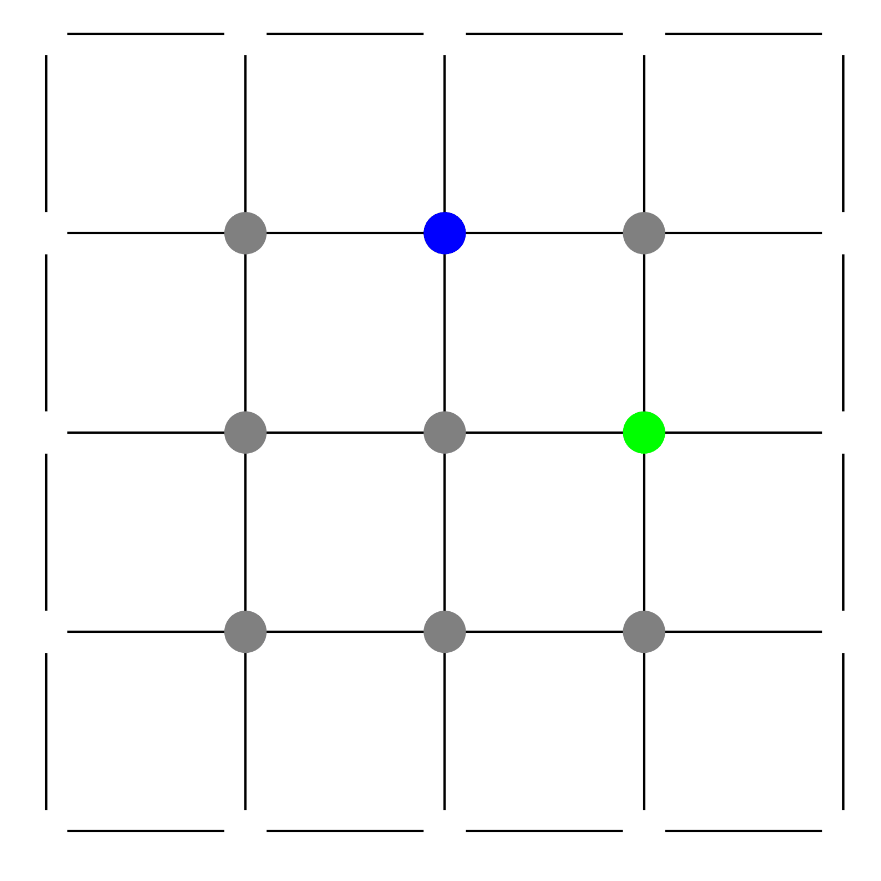
\includegraphics[height=15em]{petal-walk-1-world-crop.png}
\end{center}

Gridworlds are simplified, grid-like environments in which each \textit{cell} of the grid may be assigned a \textit{label}. In the example above, these labels are \textcolor{green}{agent}, \textcolor{blue}{object}, \textcolor{gray}{floor}, and wall. Such environments can be used to test and develop AI algorithms, particularly in reinforcement learning \cite{Leike:2017}.
\end{posterbox}

%----------------------------------------------------------------------------------------
%	Reconfigurable systems
%----------------------------------------------------------------------------------------

\begin{posterbox}[
    name = reconfigsys,  % Name for alignment 
    column = 1, % Column 
    ]{3. Reconfigurable}
    
Ghrist \& Peterson \cite{Ghrist-Peterson:2007} define reconfigurable systems as a collection of labels on a graph, where local rearrangements of the labels represent reconfigurations of the system.
\vspace{0.15cm}

From \cite{Ghrist-Peterson:2007}: $G$ is a graph. $A$ is a set of possible labels on the vertices of $G$.
\vspace{0.15cm}

A \textit{generator} $\phi$ is a collection of three objects:
\begin{itemize}
    \item the \textit{support}, $SUP(\phi) \subset G$
    \item the \textit{trace}, $TR(\phi) \subset SUP(\phi)$
    \item a \textit{relabelling} for the vertex set $TR(\phi)$
\end{itemize}
\end{posterbox}

%----------------------------------------------------------------------------------------
%	State Complexes
%----------------------------------------------------------------------------------------

\begin{posterbox}[
    name = scs,  % Name for alignment 
    column = 1, % Column 
    aligned=references,
    below=reconfigsys,
    above=futureresearch
    ]{4. State Complexes Research}
    
\begin{center}
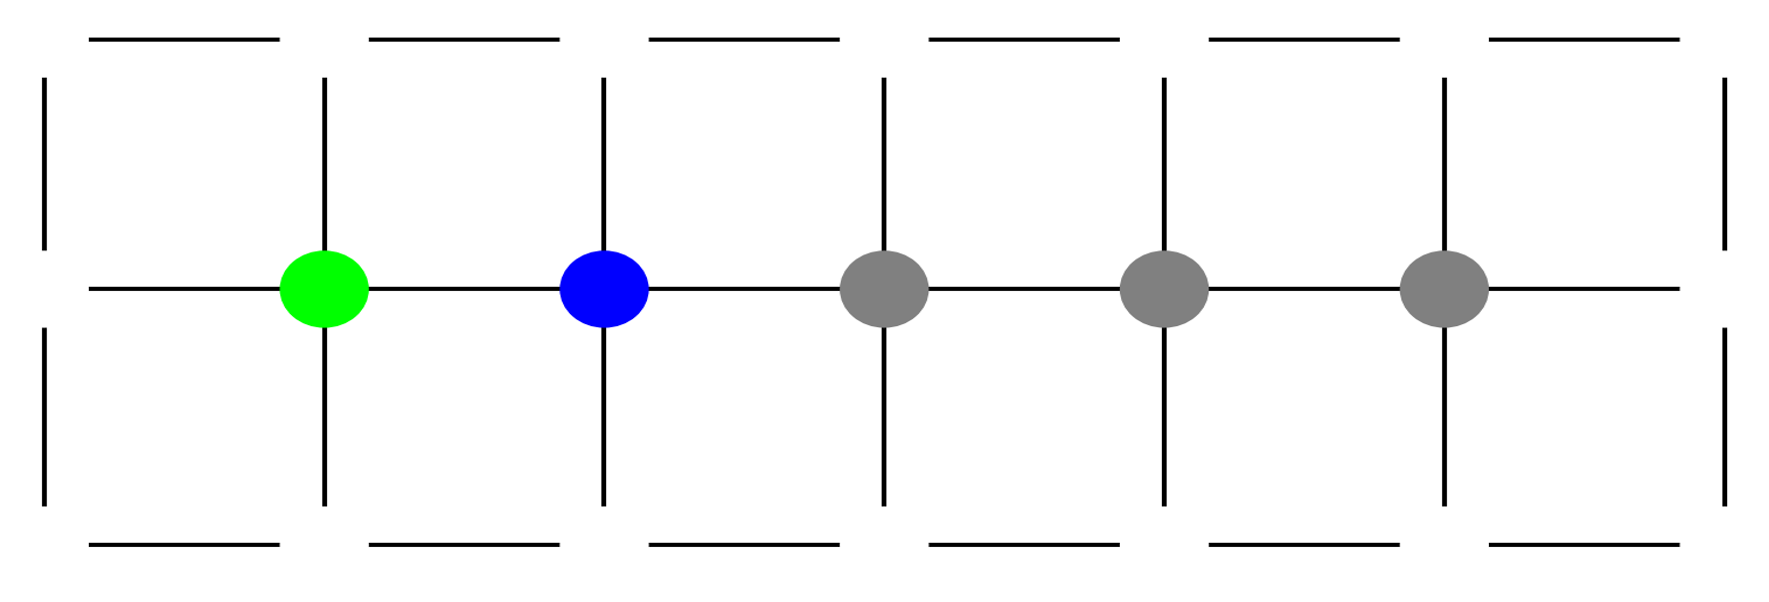
\includegraphics[width=0.8\textwidth]{coorridor.PNG}
\vspace{0.15cm}

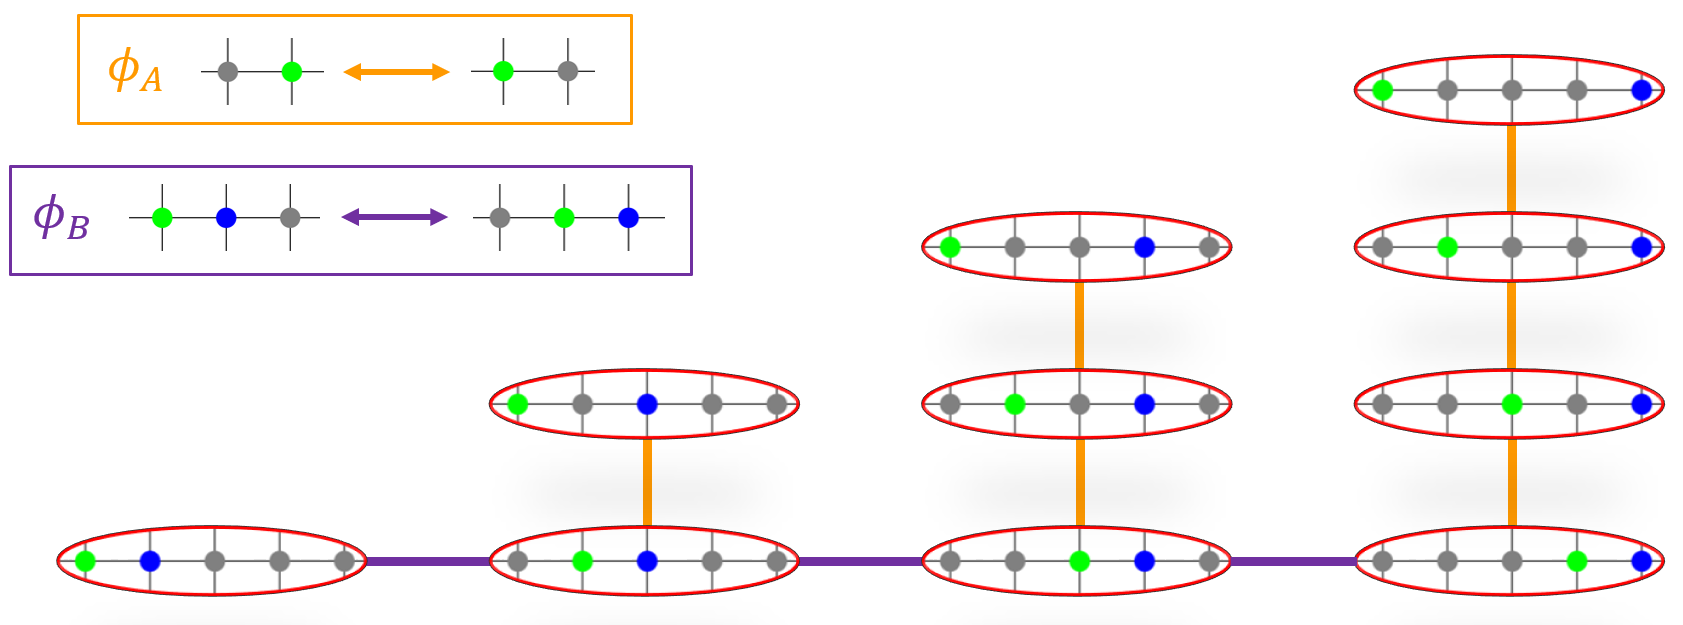
\includegraphics[width=1\textwidth]{SC-example.PNG}
\vspace{-0.25cm}
\end{center}

Ghrist \& Peterson \cite{Ghrist-Peterson:2007} define a \textcolor{red}{state} of a reconfigurable system as a choice of labels (chosen from $A$) for every vertex of $G$.
\vspace{0.15cm}

$\textcolor{red}{s_i}:V(G) \rightarrow A$
\vspace{0.15cm}

The state complex $S$ is a graph with vertices corresponding to states, with edges connecting a pair states differing by a single generator.
\end{posterbox}


%----------------------------------------------------------------------------------------
%	State Complexes of Gridworlds
%----------------------------------------------------------------------------------------

\begin{posterbox}[
    name = scsofgrids,  % Name for alignment 
    column = 2, % Column 
    span = 2,
    bottomaligned=grid,
    above=references
    ]{5. State Complexes of Gridworlds}
    
\begin{center}
    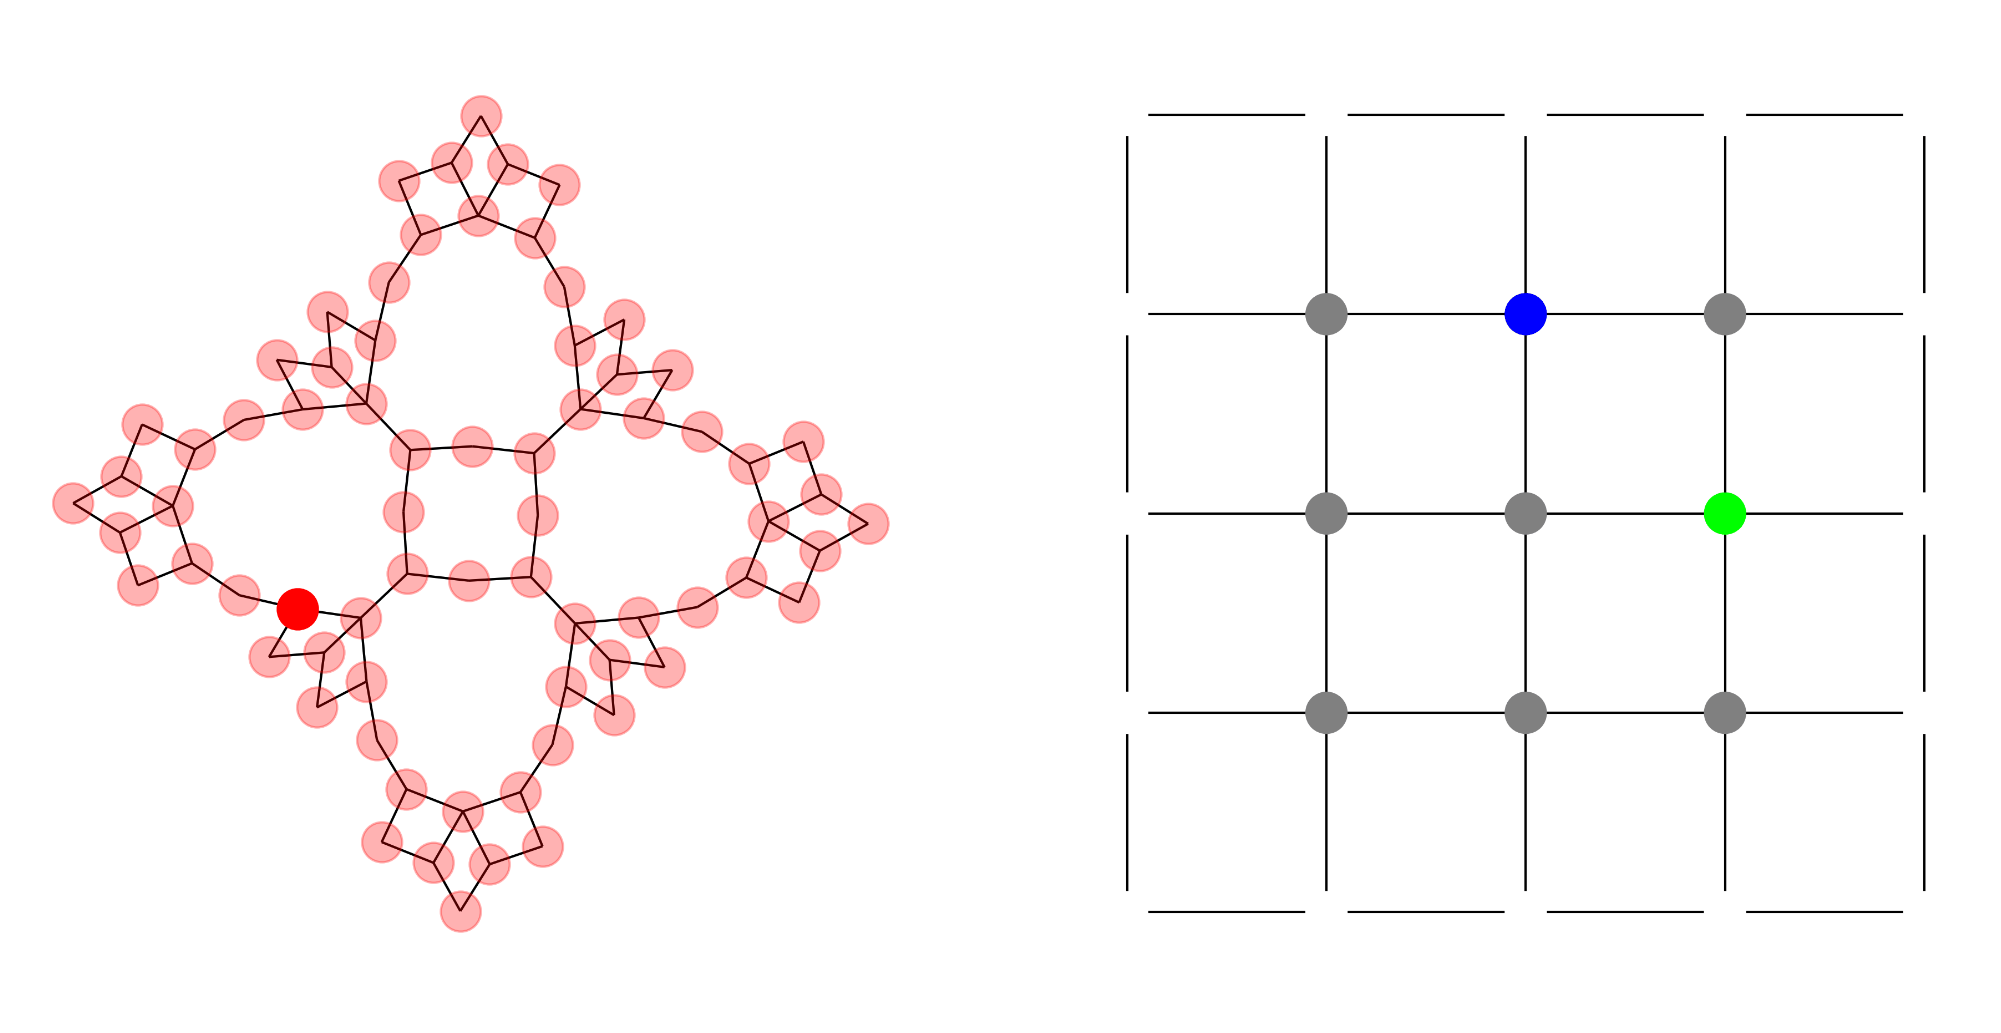
\includegraphics[width=0.9\textwidth]{petal-walk-1.PNG}
\end{center}

State complexes often capture symmetries in a gridworlds' geometry or labelling, as shown in these examples. The petal-like state complex above shows different scales of geometry; for each position of the \textcolor{blue}{object} there exists a subgraph of 8 verticies (representing the 8 possible locations of the \textcolor{green}{agent}) which is connected to as many other subgraphs as is possible for the \textcolor{green}{agent} to push or pull the \textcolor{blue}{object} to a different location from the current location represented in that subgraph.

\vspace{0.6cm}
\begin{center}
    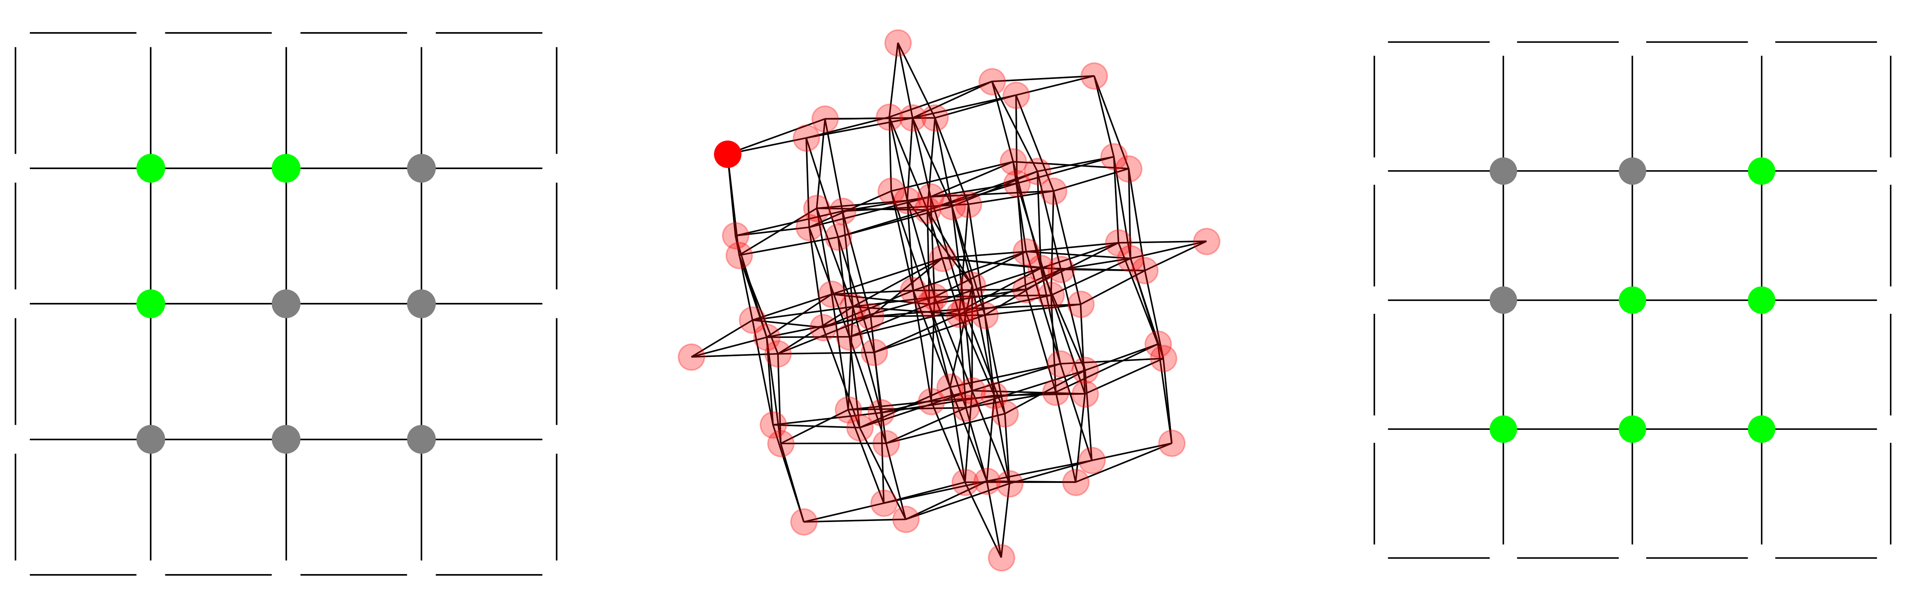
\includegraphics[width=1\textwidth]{3-6-agents.PNG}
\end{center}
\end{posterbox}

\end{poster}
\end{document}